\usetikzlibrary{chains}
\begin{frame}{exercise 1} 
\begin{tikzpicture}
\begin{scope}[start chain=going right,node distance=0mm,every node/.style={on chain,draw,font=\small,minimum height=1cm}]
\node (opcode) { opcode }; \node[dashed] { mod | reg{\fontsize{9}{10}\selectfont/opcode} | r/m}; \node[dashed] {scale / idx / base}; \node[dashed] {displacement}; \node[dashed] {immediate};
\end{scope}
\node[anchor=north west] (modrmtbl) at (opcode.south west) {
    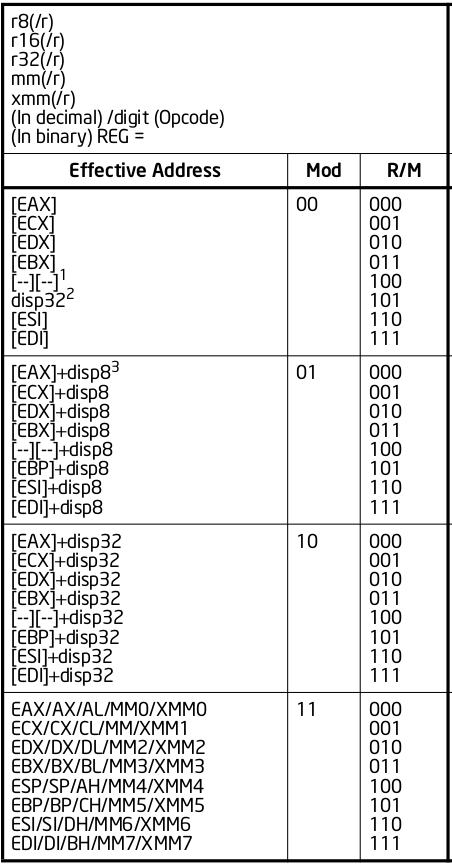
\includegraphics[height=0.8\paperheight]{../x8664-encoding/32bitmodrm}
};
\node[anchor=north west] (bts manual)at (modrmtbl.north east) {
    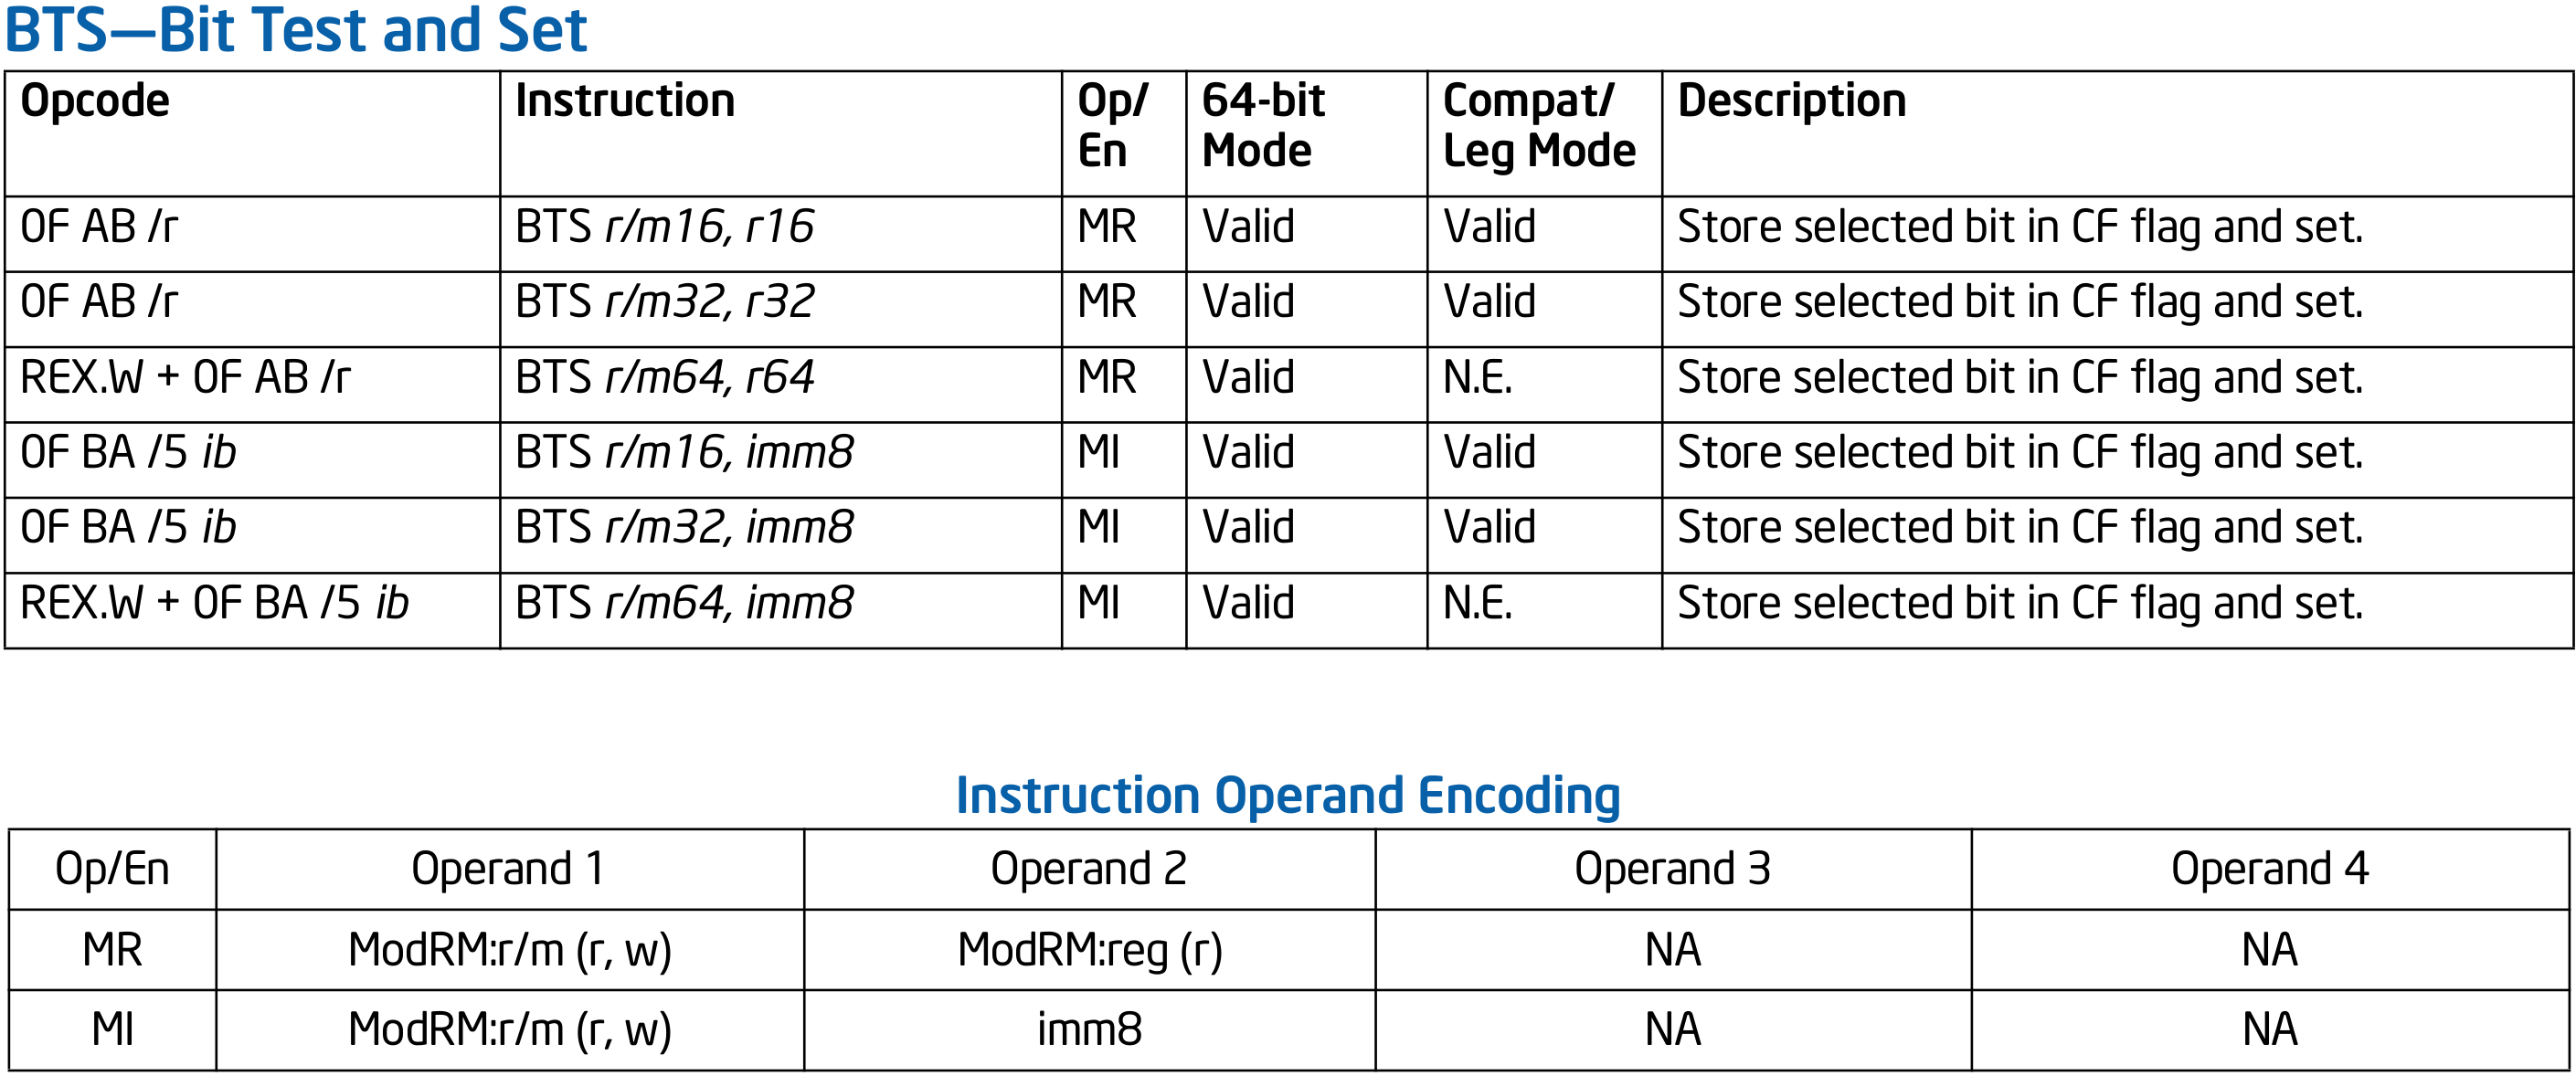
\includegraphics[width=0.75\textwidth]{../x8664-encoding/bts-manual}
};
\node[anchor=north west,align=left] (bts ex) at (bts manual.south west) {
    exercise: encode \texttt{btsl \$7, 4(\%rax)} \\
    (Intel syntax: \texttt{BTS DWORD PTR[RAX+4], 7})
};
\end{tikzpicture}
\end{frame}
